
\documentclass[
	% -- opções da classe memoir --
	article,			% indica que é um artigo acadêmico
	11pt,				% tamanho da fonte
	oneside,			% para impressão apenas no verso. Oposto a twoside
	a4paper,			% tamanho do papel. 
	% -- opções da classe abntex2 --
	%chapter=TITLE,		% títulos de capítulos convertidos em letras maiúsculas
	%section=TITLE,		% títulos de seções convertidos em letras maiúsculas
	%subsection=TITLE,	% títulos de subseções convertidos em letras maiúsculas
	%subsubsection=TITLE % títulos de subsubseções convertidos em letras maiúsculas
	% -- opções do pacote babel --
	english,			% idioma adicional para hifenização
	brazil,				% o último idioma é o principal do documento
	sumario=tradicional
	]{abntex2}


%\newcommand{\matlabCodePath}{/home/clifte/git/Mestrado/Matlab/}
 
\newcommand{\matlabCodePath}{C:/Users/clifte/git/mestrado/Matlab/} 

\newcommand{\matlabRBFCodePath}{\matlabCodePath Trabalho_RNA/trabalho2/RBF/}
\newcommand{\matlabMLPCodePath}{\matlabCodePath Trabalho_RNA/trabalho2/MLP/}
\newcommand{\matlabOLAMCodePath}{\matlabCodePath Trabalho_RNA/trabalho2/OLAM/}
\newcommand{\matlabELMCodePath}{\matlabCodePath Trabalho_RNA/trabalho2/ELM/}
\newcommand{\matlabSOMCodePath}{\matlabCodePath Trabalho_RNA/trabalho2/SOM/}
% ---
% PACOTES 
% ---

% ---
% Pacotes fundamentais 
% ---
\usepackage{lmodern}			% Usa a fonte Latin Modern
\usepackage[T1]{fontenc}		% Selecao de codigos de fonte.
\usepackage[utf8]{inputenc}		% Codificacao do documento (conversão automática dos acentos)
\usepackage{indentfirst}		% Indenta o primeiro parágrafo de cada seção.
\usepackage{nomencl} 			% Lista de simbolos
\usepackage{color}				% Controle das cores
\usepackage{graphicx}			% Inclusão de gráficos
\usepackage{microtype} 			% para melhorias de justificação
 
\usepackage{amsmath} 			% Equações 
\usepackage{graphicx}
\usepackage{caption}
\usepackage{subcaption}
\usepackage{tikz}
\usepackage{listings}
\usepackage[]{mcode}
\usepackage{listingsutf8}
\usepackage{epstopdf}
\usepackage{csvsimple}


% ---
		
% ---
% Pacotes adicionais, usados apenas no âmbito do Modelo Canônico do abnteX2
% ---
\usepackage{lipsum}				% para geração de dummy text
% ---
		
% ---
% Pacotes de citações
% ---
\usepackage[brazilian,hyperpageref]{backref}	 % Paginas com as citações na bibl
\usepackage[alf]{abntex2cite}	% Citações padrão ABNT


% ---

% ---
% Configurações do pacote backref
% Usado sem a opção hyperpageref de backref
\renewcommand{\backrefpagesname}{Citado na(s) página(s):~}
% Texto padrão antes do número das páginas
\renewcommand{\backref}{}
% Define os textos da citação
\renewcommand*{\backrefalt}[4]{
	\ifcase #1 %
		Nenhuma citação no texto.%
	\or
		Citado na página #2.%
	\else
		Citado #1 vezes nas páginas #2.%
	\fi}%
% ---

% ---
% Informações de dados para CAPA e FOLHA DE ROSTO
% ---
\titulo{Relatório de Trabalho 2}
\autor{David Clifte da Silva Vieira}
\local{Brasil}
\data{2014, 21 de outubro}
% ---

% ---
% Configurações de aparência do PDF final

% alterando o aspecto da cor azul
\definecolor{blue}{RGB}{41,5,195}

% informações do PDF
\makeatletter
\hypersetup{
     	%pagebackref=true,
		pdftitle={\@title}, 
		pdfauthor={\@author},
    	pdfsubject={Modelo de artigo científico com abnTeX2},
	    pdfcreator={LaTeX with abnTeX2},
		pdfkeywords={abnt}{latex}{abntex}{abntex2}{atigo científico}, 
		colorlinks=true,       		% false: boxed links; true: colored links
    	linkcolor=blue,          	% color of internal links
    	citecolor=blue,        		% color of links to bibliography
    	filecolor=magenta,      		% color of file links
		urlcolor=blue,
		bookmarksdepth=4
}
\makeatother
% --- 

% ---
% compila o indice
% ---
\makeindex
% ---

% ---
% Altera as margens padrões
% ---
\setlrmarginsandblock{3cm}{3cm}{*}
\setulmarginsandblock{3cm}{3cm}{*}
\checkandfixthelayout
% ---

% --- 
% Espaçamentos entre linhas e parágrafos 
% --- 

% O tamanho do parágrafo é dado por:
\setlength{\parindent}{1.3cm}

% Controle do espaçamento entre um parágrafo e outro:
\setlength{\parskip}{0.2cm}  % tente também \onelineskip

% Espaçamento simples
\SingleSpacing

% ----
% Início do documento
% ----
\begin{document}
% Retira espaço extra obsoleto entre as frases.


% ----------------------------------------------------------
% ELEMENTOS PRÉ-TEXTUAIS
% ----------------------------------------------------------

%---
%
% Se desejar escrever o artigo em duas colunas, descomente a linha abaixo
% e a linha com o texto ``FIM DE ARTIGO EM DUAS COLUNAS''.
% \twocolumn[    		% INICIO DE ARTIGO EM DUAS COLUNAS
%
%---
% página de titulo
\maketitle
\frenchspacing 


% ]  				% FIM DE ARTIGO EM DUAS COLUNAS
% ---

% ----------------------------------------------------------
% ELEMENTOS TEXTUAIS
% ----------------------------------------------------------
\textual

% ----------------------------------------------------------
% Introdução
% ----------------------------------------------------------
\section*{Introdução}
\addcontentsline{toc}{section}{Introdução}
Este trabalho apresenta o resultados obtidos durante o desenvolvimento da
segunda lista de exercícios propostos pelo professor Ajalmar Roccha no curso de
mestrado em Ciências da Computação do IFCE. Parte do código fonte é exibido na
forma de Apêndice ao fim do trabalho. Foram abordados as redes RBF, ELM, MLP,
OLAM e SOM. Ao final de sessão temos o resultado obtido pelas redes.


\section*{OLAM – Optimal Linear Associative Memory} 
O OLAM foi proposto por
Kohonen and Ruohonen \cite{OLAM_1}. É um classificador linear muito utilizado
seja sozinho para realizar classificações lineares como em conjunto com outras
redes como ELM e RBF. A OLAM é um modelo que permite uma recuperação das
informações assossiadas na memória $\{y_k,k=1,2,\ldots,n|y_k\in Y\}$ a partir de
um $x_k$ desde que o conjunto $\{x_k,k=1,2,\ldots,m|x_k \in X\}$ seja
linearmente independente, diferentemente de outras tecnicas de memória
associativa que exigem que o conjunto seja ortogonal.\\
Para que essa recuperação a partir de $x_k$ seja possível é necessário que a
matriz $W$ satisfaça a seguinte equação:
\begin{align}
Y=WX
\end{align}
Para o caso de $m=n$ e os valores da matriz $X$ sejam linearmente independentes
podemos computar o valor de $W$ da mesma forma que resolvemos um sistema de
equações lineares:
\begin{align}
W*=YX^{-1}
\end{align}
O que obriga que a matriz $X$ possua uma inversa. Desta forma é possível
recuperar qualquer valor de $y_k$ dado um $x_k$.
\\
Para $m \neq n$ o cálculo da inversa não pode ser realizado, tendo em vista que
a matriz não é quadada. Para superar tal característica pode-se utilizar a
pseudo-inversa de $X$, $X^{\dagger}$, desde que que $XX^T$ seja inversível. A
pseudo-inversa está definidada no trabalho de \cite{penrose_1}.

\begin{align}
W*=Y(X^TX)^{-1}X^T
\end{align}
\subsection*{Resultados obtidos}
Abaixo temos o resultado obtido ao utilizar o classificador linear, OLAM.
A acurácia foi obtida após o teste com 50 iterações.

\begin{table}[h]
\centering
	\begin{tabular}{|l|l|l|l|l|l|}
	\hline
	DataSet          & Acurácia & nTreinamento & nTeste \\ \hline
	Íris             & 0.8324   & 112          & 38     \\\hline 
	Derme     		 & 0.9642   & 274          & 92     \\ \hline
	Coluna Vertebral & 0.7873   & 232          & 78     \\
	\hline
	\end{tabular}
	\caption{Acurácia obtida para os três conjuntos de dados utilizando o
	OLAM.nTreinamento e nTeste são as quantidades de dados de
	treinamento e quantidade de dados de teste utilizados}
\end{table}  
   

\begin{table}[h]
\centering
\csvreader[tabular=|c|c|c|c|,
		   separator=tab,
		   late after line={\\\hline},
		   no head, table head=\hline
		   ]
{\matlabOLAMCodePath saida/OLAM_confusion_iris.csv} {}
{\csvcoli & \csvcolii & \csvcoliii & \csvcoliv}
\caption{Matriz confusão obtida para a base da iris utilizando o OLAM}
\end{table} 
     
  


\begin{table}[h]
\centering
\csvreader[tabular=|p{2cm}|l|p{1.8cm}|p{1.5cm}|p{1.8cm}|p{1.8cm}|p{1.8cm}|,
		   separator=tab,
		   late after line={\\\hline},
		   no head, table head=\hline
		   ]
{\matlabOLAMCodePath saida/OLAM_confusion_derme.csv} {}
{\csvcoli & \csvcolii & \csvcoliii & \csvcoliv & \csvcolv & \csvcolvi}
\caption{Matriz confusão obtida para a base da derme utilizando o OLAM}
\end{table} 


 
\begin{table}[h]
\centering
\csvreader[tabular=|c|c|c|c|,
		   separator=tab,
		   late after line={\\\hline},
		   no head, table head=\hline
		   ]
{\matlabOLAMCodePath saida/OLAM_confusion_vertebra.csv} {}
{\csvcoli & \csvcolii & \csvcoliii & \csvcoliv}
\caption{Matriz confusão obtida para a base da vertebra utilizando o OLAM}
\end{table} 
     

\section*{RBF - Radial Basis Function}

\subsection{Teorema de Cover} As redes RBF tem como princípio a transformação
não linear das entradas para um espaço de alta dimensionalidade. Segundo o
teorema de Cover sobre a separabilidade de padrões, nesse novo espaço de alta
dimensionalidade a probabilidade de existir um hiperplano que posso separar
linearmente os dados é maior.

\begin{citacao}
Um problema complexo de classificação de padrões disposto não linearmente em um
espaço de alta dimensão tem maior probabilidade de ser linearmente separável do
que em um espaço de baixa dimensionalidade.(Cover, 1965) 
\end{citacao}

\begin{align}
P(N,m_1) = \left(\frac{1}{2}\right)^{N-1}   
\sum_{m=0}^{m_1-1}   
\binom{N-1}{m}
\label{eq:teoSepCover}
\end{align}

Na equação \ref{eq:teoSepCover}, citada no trabalho de Cover temos a
probabilidade de um padrão $x$ ser separado linearmente de $\chi=\{x_i\}_{i=1}^{N}$ após passar por uma
transformação através de uma função oculta $\phi(x)$ que mapeia o padrão $x$ em
um espaço de maior dimensionalidade.
Podemos perceber que a medida que o número de dimensões $m_1$ aumentam para uma
determinado número $N$ padrões a probabilidade resultante tende a 1.


\subsection{Mapeamento da função oculta}
Um mapeamento não linear é utilizado para realizar uma tranfomação nos dados de
classificação de forma que ele possa ser resolvido linearmente. Como visto na
sessão anterior, Cover resolveu este problema ao aumentar o número de dimensões
dos padrões.

O mapeamento é feito através do vetor $\phi(x)$.
\begin{align}
\phi(x) = [ \phi_1(x), \phi_2(x), \ldots, \phi_{m1}(x) ] 
\label{eq:phiVec}
\end{align}
Dado um vetor $x$ oriundo do espaço de entrada de dimensão $m_0$. O vetor
$\phi(x)$ realiza o mapeamento de $x$ em novo espaço de dimensão $m_1$. Como
representado na equação \ref{eq:phiVec}, $\phi(x)$ é um conjunto de funções
ocultas $\{\phi_i(x)\}^{m_1}_{i=1}$ que mapeiam o vetor $x$ no novo espaço
denominado espaço oculto ou espaço de caracaterísticas. É esperado que no espaço
de características seja possível realizar a classificação dos dados de forma
linear. O hiperplano que separa as classes é definido por
\begin{align}
\phi(x)W^t=0
\end{align} 

Desta forma temos que para $x \in \chi_1 $, $\phi(x)W^t>0$, onde $W$ é um
vetor com os termos da combinação das funções de base radial e $\chi_1$ é a
classe na qual $x$ faz parte.

\subsection{A Rede RBF}
Uma rede RBF(Radial Basis function), da mesma forma que rede MLP e ELM é
composta por três camadas.
Uma camada de entrada, camada oculta e camada de saída. A principal diferença entre
este modelo e os outros está na camada oculta que apresenta como função de
ativação uma função de base radial.

Uma função de base radial é caracterizada pelo valor aumentar ou
diminuir de acordo com a distancia ao ponto central da função. A função
gaussiana geralmente é utilizadas em redes RBFs, ela se caracteriza por valores
próximos da média apresentarem valores próximos a 1 e valores distantes da média
apresentam valores próximos a 0. Através do valor da variância é
possível controlar o raio de atuação da gaussiana como função de base
radial.

A resposta a uma entrada $x$ em uma rede RBF pode ser representada como:
\begin{align}
Y(X)=\sum^{N}_{i=1}W_i\phi(\|x-x_i\|)
\end{align}

\subsection{Treinamento da rede}
O treinamento de uma rede RBF possui duas fases. A princípio é necessário
definir os parâmetros das funções de base radial e posteriormente os pesos
utilizados nos neurônios de saída. Uma técnica geralmente utilizada para a
definição dos parâmetros das funções de base radial é o K-means, nele K
vetores médios pertecentes aos dados de treinamentos são escolhidos como centro
das funções de base radial(Bishop, 1995). Uma outra abordagem possível para a
definição dos centros das funções é realizar a subamostragem dos vetores de
entrada. Após a definição das funções de base radial resta apenas o calculo dos
pesos da camada de saída. Como dito anteriormente este problema se resume a
otimização de um classificador linear e pode ser obtido com a tecnica simples
da pseudo inversa (Haykin, 2008).
\begin{align}
W\phi=Y \\
W*\phi*\phi^{-1}=Y*\phi^{-1}\\
W=Y*\phi^{-1},\ para\ \phi\ quadrado\ ou \\
W=Y*\phi^{\dagger},\ para\ \phi\ não\ quadrado
\end{align}

\subsection{Exemplo de aplicação de uma rede RBF}
A Rede RBF será aplicada para problemas de classificação, são eles:
Problemas da iris, doenças de pele e da coluna vertebral. Para todos os
problemas a determinação dos parâmetros da rede foi feita através do algoritmo
de otimização gridSearch. Foram variados os valores de sigma e da quantidade de
neurônios afim de se obter o melhor resultado para cada problema.
Foram obtidos os seguintes resultados para os três conjuntos de dados, tabela
\ref{tab:rbfRes}.

\begin{table}[h]
\centering
\begin{tabular}{|l|l|l|l|l|l|}
\hline
DataSet          & Acurácia & nTreinamento & nTeste & nNeurônios & Sigma \\ \hline
Íris             & 0,9533   & 120          & 30     & 8          & 4,85  \\ \hline
Derme            & 0,9068   & 292          & 73     & 10         & 1,85  \\ \hline
Coluna Vertebral & 0,8226   & 248          & 62     & 12         & 4,10   \\
\hline
\end{tabular}

\caption{Resultados obtidos pelo classificador RBF.nTreinamento, nTeste e
nNeurônios são as quantidades de dados de treinamento, quantidade de dados
de teste e quantidade de neurônios utilizados no treinamento. Sigma é o valor
de sigma utilizado na gaussiana multivariada.}
\label{tab:rbfRes}
\end{table} 
 
Foi obtido também a matriz confusão para cada conjunto de dados. Na tabela
\ref{tab:confRBFIris} temos a matriz confusão resultante do teste do treinamento
na base de dados da íris, podemos observar que há uma pequena confusão entre as
classes versicolor e virgínica. Podemos verificar nas tabelas
\ref{tab:confRBFDerme}, \ref{tab:confRBFVertebra} algo semelhante, pequenas
confusões entre as classes mais próximas.

\begin{table}[h]
\centering
\csvreader[tabular=|c|c|c|c|,
		   separator=tab,
		   late after line={\\\hline},
		   no head, table head=\hline
		   ]
{\matlabRBFCodePath saida/RBF_confusion_iris.csv} {}
{\csvcoli & \csvcolii & \csvcoliii & \csvcoliv}
\caption{Matriz confusão obtida para a base da iris utilizando o RBF}
\label{tab:confRBFIris}
\end{table} 
     
\begin{table}[h] 
\centering
\csvreader[tabular=|p{2cm}|l|p{1.8cm}|p{1.5cm}|p{1.8cm}|p{1.8cm}|p{1.8cm}|,
		   separator=tab,
		   late after line={\\\hline},
		   no head, table head=\hline
		   ] 
{\matlabRBFCodePath saida/RBF_confusion_derme.csv} {}
{\csvcoli & \csvcolii & \csvcoliii & \csvcoliv & \csvcolv & \csvcolvi &
\csvcolvii}
\caption{Matriz confusão obtida para a base de dados de doenças da derme
utilizando o RBF}
\label{tab:confRBFDerme}
\end{table}



\begin{table}[h]
\centering
\csvreader[tabular=|c|c|c|c|,
		   separator=tab,
		   late after line={\\\hline},
		   no head, table head=\hline
		   ]
{\matlabRBFCodePath saida/RBF_confusion_vertebra.csv} {}
{\csvcoli & \csvcolii & \csvcoliii & \csvcoliv}
\caption{Matriz confusão obtida para a base de dados de doenças da coluna
utilizando o RBF}
\label{tab:confRBFVertebra}
\end{table}
 


 \section*{ELM - Extreme Learning
Machines} As redes ELM são redes baseadas em apenas uma camada oculta, assim como a
rede RBF e a MLP as entradas são propagadas progressivamente até a camada de
saída.Proposta por Huang et al \cite{ELM_25}, \cite{ELM_67} tem como finalidade
superar os problemas encontrados nas redes baseadas no gradiente descendente
como o Backpropagation aplicado no MLP.
O ELM reduz consideravelmente o tempo necessário para o treinamento da rede
neural pois possui uma maneira única de determinação da memória da rede. A
redução no tempo de treinamento é ocasionada pela não atualização dos pesos da
camada oculta. Os pesos das sinapses desta camada são atribuídos aleatóriamente
e não são alterados durante o treinamento, desta forma apenas a camada de saída
tem seus pesos atualizados.
\\
Não há restrições quanto a função de ativação da camada oculta de uma rede ELM,
contanto que a função não seja linear. A exemplo da utilização de funções de
base radial, pode-se utilizar valores aleatórios para os parâmetros destas
funções.
Como todos os parâmetros da rede ELM são definidos de forma aleatória durante o
treinamento restam para o treinamento apenas os ajustes dos parâmetros e pesos
da camada oculta. Para tanto pode-se utilizar o OLAM para realizar estes
ajustes. A saída da rede ELM pode ser computada da seguinte forma:
\begin{align}
	U_h=f(X  W_h) \\
	Yc=U_h  W_o
\label{eq:logistica}
\end{align}
Para o treinamento devemos apenas calcular a matriz $W_o$. Para isso levamos em
consideração apenas a saída gerada pela camada oculta $U_h$ e as saídas
desejadas $Y_d$.
\begin{align}
	Yc = U_h  W_o \\
	W_o = U_h^\dagger Y_d
\label{eq:logistica}
\end{align}

\subsection*{Resultados obtidos}
Abaixo, figura \ref{tab:elm_iris},\ref{tab:elm_derme} e \ref{tab:elm_vertebra}
temos o resultado obtido ao utilizar o classificador ELM.
A acurácia foi obtida após o teste com 50 iterações.

\begin{table}[h]
\centering
	\begin{tabular}{|l|l|l|l|l|l|}
	\hline
	DataSet          & Acurácia & nTreinamento & nTeste& nNeurônios \\ \hline
	Íris             & 0.9409   & 127          & 22    & 27 \\\hline 
	Derme     		 & 0.6725   & 275          & 91    & 51 \\ \hline
	Coluna Vertebral & 0.8152   & 263          & 46    & 27 \\
	\hline
	\end{tabular}
	\caption{Resultados obtidos pelo classificador ELM.nTreinamento, nTeste e
nNeurônios são as quantidades de dados de treinamento, quantidade de dados
de teste e quantidade de neurônios utilizados no treinamento. }
\end{table}  
   

\begin{table}[h]
\centering
\csvreader[tabular=|c|c|c|c|,
		   separator=tab,
		   late after line={\\\hline},
		   no head, table head=\hline
		   ]
{\matlabELMCodePath saida/ELM_confusion_iris.csv} {}
{\csvcoli & \csvcolii & \csvcoliii & \csvcoliv}
\caption{Matriz confusão obtida para a base da iris utilizando o ELM}
\label{tab:elm_iris}
\end{table} 
     
  


\begin{table}[h]
\centering
\csvreader[tabular=|p{2cm}|l|p{1.8cm}|p{1.5cm}|p{1.8cm}|p{1.8cm}|p{1.8cm}|,
		   separator=tab,
		   late after line={\\\hline},
		   no head, table head=\hline
		   ]
{\matlabELMCodePath saida/ELM_confusion_derme.csv} {}
{\csvcoli & \csvcolii & \csvcoliii & \csvcoliv & \csvcolv & \csvcolvi}
\caption{Matriz confusão obtida para a base da derme utilizando o ELM}
\label{tab:elm_derme}
\end{table} 


 
\begin{table}[h]
\centering
\csvreader[tabular=|c|c|c|c|,
		   separator=tab,
		   late after line={\\\hline},
		   no head, table head=\hline
		   ]
{\matlabELMCodePath saida/ELM_confusion_vertebra.csv} {}
{\csvcoli & \csvcolii & \csvcoliii & \csvcoliv}
\caption{Matriz confusão obtida para a base da vertebra utilizando o ELM}
\label{tab:elm_vertebra}
\end{table} 
     

\section*{MLP - Multilayer Perceptron}

Uma rede MLP é uma rede multicamada constituída por perceptrons conectados
entre si por pesos. Os perceptrons pertencentes a rede estão conectados formando
pelo menos três camadas. A primeira é a camada de entrada, responsável por
receber os sinais de entrada, processá-lo e encaminhá-los para a camada oculta.
A segunda camada, chamada de camada oculta realiza o processamento dos dados
vindos da camada de entrada e encaminha o resultado para a camada seguinte esta
podendo ser outra camada oculta ou a camada de saída. Finalmente a camada de
saída que representa o resultado da rede. 

\begin{figure}[!htb]
	\centering
	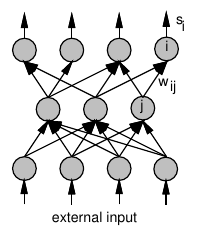
\includegraphics[width=6cm]{imagens/mlp.png}
	\caption{Rede MLP.}
	\label{fig:digraph}
\end{figure}

Na figura \ref{fig:digraph} temos uma representação de uma rede MLP.
onde $s_i$ é a camada calculada, $s_j$ é a camada anterior, $w_j$ são os pesos
da conexão e $f$ é a função de ativação do neurônio. A função de ativação
costuma ser uma sigmoíde como a tangente hiperbólica ou a logística, porém o
mais importante desta função é que ela seja diferenciável. Isso será uma
característica importante para o algoritmo Backpropagation Na equação
\ref{eq:logistica} e \ref{eq:logisticaDer} temos a função sigmóide logística e
sua derivada aplicada a um perceptron.
\begin{align}
	s_i=f(s_j*w_j)=f(net_i)=\frac{1}{1+e^{-net_i}}
\label{eq:logistica}
\end{align}

\begin{align}
	f'(s_i)=s_i*(1-s_i)
\label{eq:logisticaDer}
\end{align} 

\subsection{Backpropagation}
Durante a fase de treinamento a atualização dos pesos de forma geral é feita de
acordo com a equação \ref{eq:atualPeso}
\begin{align}
	\Delta w(t)= \eta*\frac{\delta E}{\delta w} \\
	w(t+1)=w(t)+\Delta w(t)
\label{eq:atualPeso}
\end{align}
A ideia principal do backpropagation é calcular as derivadas parcias
$\frac{\delta E}{\delta w}$ para cada peso da rede. Isso é feito através da
aplicação sucessiva da regra da cadeia.
\begin{align}
\frac{\delta E}{\delta w_{ij}}=
\frac{\delta E}{\delta s_i}
\frac{\delta s_i}{\delta w_{ij}}
\\ onde \\
\frac{\delta s_i}{\delta w_{ij}}=
\frac{\delta s_i}{\delta net_i}
\frac{\delta net_i}{\delta w_{ij}}=
f'(net_i)s_j
\end{align}

O cáculo de $\frac{\delta E}{\delta s_i}$, ou seja, a influencia da saída
$s_i$ no erro $E$ é diferente para a camada oculta e camada de saída.
Na camada de saída o cálculo de $\frac{\delta E}{\delta s_i}$ é feita da
seguinte forma.

\begin{align}
\frac{\delta E}{\delta s_i}=
\frac{1}{2}\frac{\delta (t_i-s_i)^2}{\delta s_i}=-(t_i-s_i)
\end{align}

Já para o cáculo da camada oculta deve-se reaplicar a regra da cadeia, desta
forma temos:

\begin{align}
\frac{\delta E}{\delta s_i}=
\sum_{k \in L_i} \frac{\delta E}{\delta s_k} \frac{\delta s_k}{\delta s_i}=
\sum_{k \in L_i} \frac{\delta E}{\delta s_k} \frac{\delta s_k}{\delta net_k}
\frac{\delta net_k}{\delta s_i}=
\sum_{k \in L_i} \frac{\delta E}{\delta s_k} f'(net_k)w_{ki}
\end{align}

Após o cálculo da derivadas parciais pode-se realizar a atualização dos pesos. A
atualização dos pesos é feita corrigindo seus valores somando ao gradiente
cálculado na direção oposta. Está técnica é chamada de Gradiente descendente.
\begin{align}
\Delta w(t)=-\eta * \bigtriangledown E(t)
\end{align}
\subsection{Resultados obtidos com o MLP Backpropagation}
Nesta sessão são exibidos os resultados obtidos pelo MLP utilizando o
Backpropagation como técnica de treinamento.Para a obtenção da quantidade de
neurônios da camada oculta foi realizado o grid search com valores variando de 2
até 20. A taxa de aprendizagem foi fixada em 0.01 e a acurácia foi calculada com
base em 10 iterações.

\begin{figure} 
	\centering
	\begin{subfigure}[b]{0.4\textwidth}
		\includegraphics[width=\textwidth]
		{\matlabMLPCodePath1_Grid_Search_iris_iris.eps}
		\caption{Resultado do grid search para o dataset da íris. Melhor resultado foi
		obtido com 13 neuônios na camada oculta.}
	\end{subfigure}
    ~
    \begin{subfigure}[b]{0.4\textwidth}
		\includegraphics[width=\textwidth]
		{\matlabMLPCodePath1_Erro_medio_quadratico_iris.eps}
		\caption{Erro quadrático médio. Perceba que o erro está em escala
		logaritimica}
	\end{subfigure}     
  \caption{Resultado do treinamento da íris utilizando o MLP}
\end{figure}


\begin{figure} 
	\centering
	\begin{subfigure}[b]{0.4\textwidth}
		\includegraphics[width=\textwidth]
		{\matlabMLPCodePath1_Grid_Search_derme_derme.eps}
		\caption{Resultado do grid search para o dataset da derme. Melhor resultado
		foi obtido com 17 neuônios neuônios na camada oculta.}
	\end{subfigure}
    ~
    \begin{subfigure}[b]{0.4\textwidth}
		\includegraphics[width=\textwidth]
		{\matlabMLPCodePath1_Erro_medio_quadratico_derme.eps}
		\caption{Erro quadrático médio. Perceba que o erro está em escala
		logaritimica}
	\end{subfigure}     
  \caption{Resultado do treinamento da derme utilizando o MLP}
\end{figure}


\begin{figure} 
	\centering
	\begin{subfigure}[b]{0.4\textwidth}
		\includegraphics[width=\textwidth]
		{\matlabMLPCodePath1_Grid_Search_vertebra_vertebra.eps}
		\caption{Resultado do grid search para o dataset da coluna vertebral. Melhor
		resultado foi obtido com 5 neuônios neuônios na camada oculta.}
	\end{subfigure}
    ~
    \begin{subfigure}[b]{0.4\textwidth}
		\includegraphics[width=\textwidth]
		{\matlabMLPCodePath1_Erro_medio_quadratico_vertebra.eps}
		\caption{Erro quadrático médio. Perceba que o erro está em escala
		logaritimica}
	\end{subfigure}     
  \caption{Resultado do treinamento da coluna vertebral utilizando o MLP}
\end{figure}


 
\begin{table}[h]
\centering
\begin{tabular}{|l|l|l|l|l|}
\hline
DataSet          & Acurácia & nTreinamento & nTeste & nNeurônios \\ \hline
Íris             & 0,9682	&	128	&	22	& 13  \\ \hline
Derme            & 0,9630	&	311	&	54	& 17  \\ \hline
Coluna Vertebral & 0,8798	&	264	&	46	& 5   \\
\hline
\end{tabular}
\caption{Resultados obtidos pelo classificador RBF.nTreinamento, nTeste e
nNeurônios são as quantidades de de dados de treinamento, quantidade de dados
de teste e quantidade de neurônios utilizados no treinamento. Sigma é o valor
de sigma utilizado na gaussiana multivariada.}
\label{tab:rbfRes}
\end{table}   

Foi obtido também a matriz confusão para cada conjunto de dados.


\begin{table}[h]
\centering
\csvreader[tabular=|c|c|c|c|,
		   separator=tab,
		   late after line={\\\hline},
		   no head, table head=\hline
		   ]
{\matlabMLPCodePath saida/MLP_confusion_iris.csv} {}
{\csvcoli & \csvcolii & \csvcoliii & \csvcoliv}
\caption{Matriz confusão obtida para a base da iris}
\label{tab:confMLPIris}
\end{table} 
     
\begin{table}[h] 
\centering
\csvreader[tabular=|p{2cm}|l|p{1.8cm}|p{1.5cm}|p{1.8cm}|p{1.8cm}|p{1.8cm}|,
		   separator=tab,
		   late after line={\\\hline},
		   no head, table head=\hline
		   ] 
{\matlabMLPCodePath saida/MLP_confusion_derme.csv} {}
{\csvcoli & \csvcolii & \csvcoliii & \csvcoliv & \csvcolv & \csvcolvi &
\csvcolvii}
\caption{Matriz confusão obtida para a base de dados de doenças da derme}
\label{tab:confMLPDerme}
\end{table}



\begin{table}[h]
\centering
\csvreader[tabular=|c|c|c|c|,
		   separator=tab,
		   late after line={\\\hline},
		   no head, table head=\hline
		   ]
{\matlabMLPCodePath saida/MLP_confusion_vertebra.csv} {}
{\csvcoli & \csvcolii & \csvcoliii & \csvcoliv}
\caption{Matriz confusão obtida para a base de dados de doenças da coluna}
\label{tab:confMLPVertebra}
\end{table}



\subsection{RProp - Resilient backpropagation}
O algoritmo RProp tem como finalidade eliminar a influência da amplitude das
derivadas parciais na atualização do peso. O RProp faz isso ao considerar que os
pesos devem ser atualizados utilizando um valor fixo, $\Delta_{ij}$ em função
apenas da direção das derivadas parciais.

\begin{align}
\Delta w_{ij}(t) = 
\begin{cases} 
		-\Delta_{ij}(t), & \mbox{se } \frac{\delta E}{\delta w_{ij}}(t)>0 \\ 
		+\Delta_{ij}(t), & \mbox{se } \frac{\delta E}{\delta w_{ij}}(t)<0 \\
		0
\end{cases}
\end{align}

Caso o valor $\Delta$ seja constante durante todo o treinamento essa regra é
chamada de Regra Manhattan.
Caso seja variável é comum seguir a seguinte regra.

\begin{align}
\Delta^{(t)}_{ij} = 
\begin{cases} 
		\eta^+*\Delta_{ij}^{(t-1)}, & \mbox{se } 
		\frac{\delta E}{\delta w_{ij}}^{(t-1)}*
		\frac{\delta E}{\delta w_{ij}}^{(t)} >0
		\\
		\eta^-*\Delta_{ij}^{(t-1)}, & \mbox{se } 
		\frac{\delta E}{\delta w_{ij}}^{(t-1)}*
		\frac{\delta E}{\delta w_{ij}}^{(t)} <0 \\
		\Delta_{ij}^{(t-1)}
\end{cases}
\end{align}
onde
$0<\eta^-<1<\eta^+$.
No inicio do treinamento todos os valores são ajustados para $\Delta_0$. Como o
valor de $\Delta$ determina o tamanho do primeiro passo de atualizaçõ este
valor deve ser escolhido de acordo com os valores iniciais dos pesos.
Para evitar que o valor dos pesos fique muito grande, é determinado um valor
máximo para $\Delta$, $\Delta_{max}$. Os valores de $\Delta_0$ e $\Delta_{max}$
geralmente são parâmetros do treinamento.
\newline
\\
    Os valores de $\Delta$ são atualizados de acordo com os valores dos
fatores $\eta^+$ e $\eta^-$. Ambos os valores são obtidos de forma empírica. Isso impôe
uma resistência a variações grandes do gradiente.Pode ser verificado
nos trabalhos de (Martin Riedmiller,1994) que o algoritmo RProp converge mais
rápido para 5 diferentes benchmarks, cada um deles. Na tabela \ref{tab:bench}
temos o quadro comparativo dos algoritmos e benchmarks. Perceba que para o
problema das 2 espirais a solução não foi obtida

\begin{table}[h]
\centering
\begin{tabular}{|l|l|l|l|l}
\cline{1-4}
               & Backpropagation   & RProp & Speedup &  \\ \cline{1-4}
10-5-10        & 121               & 19    &    6,36     &  \\ \cline{1-4}
12-2-12        & \textgreater15000 & 322   &   46,58      &  \\ \cline{1-4}
Jogo da Trilha & 98                & 23    &    4,2     &  \\ \cline{1-4}
2 Espirais     & ...               & 4987  &    -     &  \\ \cline{1-4}
\end{tabular}
\caption{Quadro comparativo de benchmarks}
\label{tab:bench}
\end{table}



\newpage

\section*{SOM - Mapeamento auto-organizável} 
Neste tipo de rede o treinamento é feito
de forma diferente das outras redes como: MLP, ELM, OLAM. Esta rede
caracteriza-se por ter um aprendizado não supervisionado.
Isto significa que é apresentado para a rede os dados de treinamento, já os
dados com informações dos rótulos são ignorados. Usando esta rede os dados são
organizados em grupos de forma que estes grupos representam os dados que foram
passados para o treinamento. A rede SOM , também conhecida como rede de Kohonen.
 
\subsection{Estrutura}
A rede neural de Kohonen se diferencia das outras redes neurais. Possui apenas
uma camada de entrada e saída. Apenas um neurônio da camada de saída deve ser
acionado representando valor verdadeiro ou falso.
 A rede SOM é uma rede neural de 2 camadas que aceita padrões de N-dimensões
 como entrada e os mapeia para um conjunto de neurônios de saída, o qual
 representa o espaço dos dados a serem agrupados. O mapa (camada) de saída, que
 é tipicamente bi-dimensional, representa as posições dos neurônios em relação
 aos seus vizinhos. A idéia é que neurônios topologicamente próximos respondam
 de maneira semelhante a entradas semelhantes. Para isso todos neurônios da
 camada de entrada são conectados aos neurônios de saída. 
 Os passos do
 algoritmo de treinamento da SOM são:


\begin{enumerate}
  \item Inicialização dos pesos de forma aleatória
  \item Apresente de um padrão de entrada à rede.
  \item Determinação do neurônio vencedor, neurônio com o maior valor de
  ativação.
  \item Atualizaçãdo dos neurônios vizinhos ao vencedor.
  \item Redução dos fatores de aprendizagem e de alcance dos vizinhos ao
  vencedor
  \item Reapresentação do próximo padrão. 
   
\end{enumerate}
\subsection{Resultados}

Abaixo temos os resultados obtidos atravé do uso da rede SOM como classificador.
Isso foi feito através da atribuição de rótulos aos pesos de acordo com as
amostras de treinamento. O problema da derme não pode ser exibido devido a sua
grande quantidade de características porém sua acurácia é exibida na tabela
\ref{tab:resSom}

\begin{table}[h]
\centering
\begin{tabular}{|l|l|}
\hline
         & Acurácia \\\hline
derme    & 0.6484   \\\hline
iris     & 0.9459   \\\hline
vertebra & 0.7143  \\\hline
\end{tabular}
\caption{Acurácia obtida com o classificador SOM}
\label{tab:resSom}
\end{table}



\begin{figure} 
	\centering
	\begin{subfigure}[b]{0.4\textwidth}
		\includegraphics[width=\textwidth]
		{\matlabSOMCodePath2__iris.eps}
		\caption{Resultado do som para o problema da íris.}
	\end{subfigure}
    ~
    \begin{subfigure}[b]{0.4\textwidth}
		\includegraphics[width=\textwidth]
		{\matlabSOMCodePath2__vertebra.eps}
		\caption{Resultado do som para o problema da coluna vertebral.}
	\end{subfigure}     
  \caption{Resultado do som para relacionando duas características do problema
  da íris e da coluna vertebral. A cor do simbolo quadrado deve ser a mesma do
  triangulo para que a classificação esteja correta.}
\end{figure}
% --- 
% Finaliza a parte no bookmark do PDF, para que se inicie o bookmark na raiz
% ---
\bookmarksetup{startatroot}% 
% ---


\begin{citacao}

\end{citacao}


% ]  				% FIM DE ARTIGO EM DUAS COLUNAS
% ---

% ----------------------------------------------- -----------
% Referências bibliográficas
% ----------------------------------------------------------
\bibliography{pdi}
Bishop, C.M., 1995, "Neural Networks for Pattern Recognition" (first ed.),
Oxford University Press Inc., New York, USA, 482 p.
 @MISC{Riedmiller94advancedsupervised,
    author = {Martin Riedmiller},
    title = {Advanced Supervised Learning in Multi-layer Perceptrons - From Backpropagation to Adaptive Learning Algorithms},
    year = {1994} 
}
%"http://galaxy.agh.edu.pl/~vlsi/AI/backp_t_en/backprop.html"
%http://jeremykun.com/2012/12/09/neural-networks-and-backpropagation/

 
% ----------------------------------------------------------
% Glossário
% ----------------------------------------------------------
%
% Há diversas soluções prontas para glossário em LaTeX. 
% Consulte o manual do abnTeX2 para obter sugestões.
%
%\glossary

% ----------------------------------------------------------
% Apêndices
% ----------------------------------------------------------
% ---

% ----------------------------------------------------------
% Anexos
% ----------------------------------------------------------
\cftinserthook{toc}{AAA}


% ---
% Inicia os anexos
% ---
%\anexos
%\begin{anexosenv}
%\chapter{}
%\end{anexosenv}

\end{document}
